\section{Agreement}\label{sec:agreement}
%% FUNCTION: Shows that round robin achieves EFX less often in a world where agents agree more on
%% what is valuable, and compares round robin with the random baseline. Because agreement hurts
%% more with more agents, the next section turns to the number of agents.

 

 In a world with more agreement, Round Robin achieves EFX less often. Figure~\ref{fig:agreement}
shows the EFX rate against the Spearman rank correlation of the world from which the instances
are drawn, for $n=2,\dots,5$ agents with $m=3n$ goods and three levels of dispersion. All other
quantities are fixed, so the figure varies only agreement. For $n=4$ agents, $m=12$ goods and
Gini $0.52$ ($\theta=1$), the EFX rate falls from $0.741$ at Spearman $0$ to $0.515$, $0.293$ and
$0.109$ at Spearman $0.24$, $0.48$ and $0.73$, and reaches $0.000$ under full agreement. For
Gini $0.28$ ($\theta=0.5$), the rate starts higher but falls in the same way, from $0.913$ to
$0.047$. Only for Gini $0.06$ ($\theta=0.1$) does it stay at $1.000$ at every level of agreement.
Each rate rests on $R=20{,}000$ instances, and the curves are paired, since all levels of
agreement use the same random seeds (Chapter~\ref{ch:model}). This result is measured, not
proven.

\begin{figure}
    \centering
    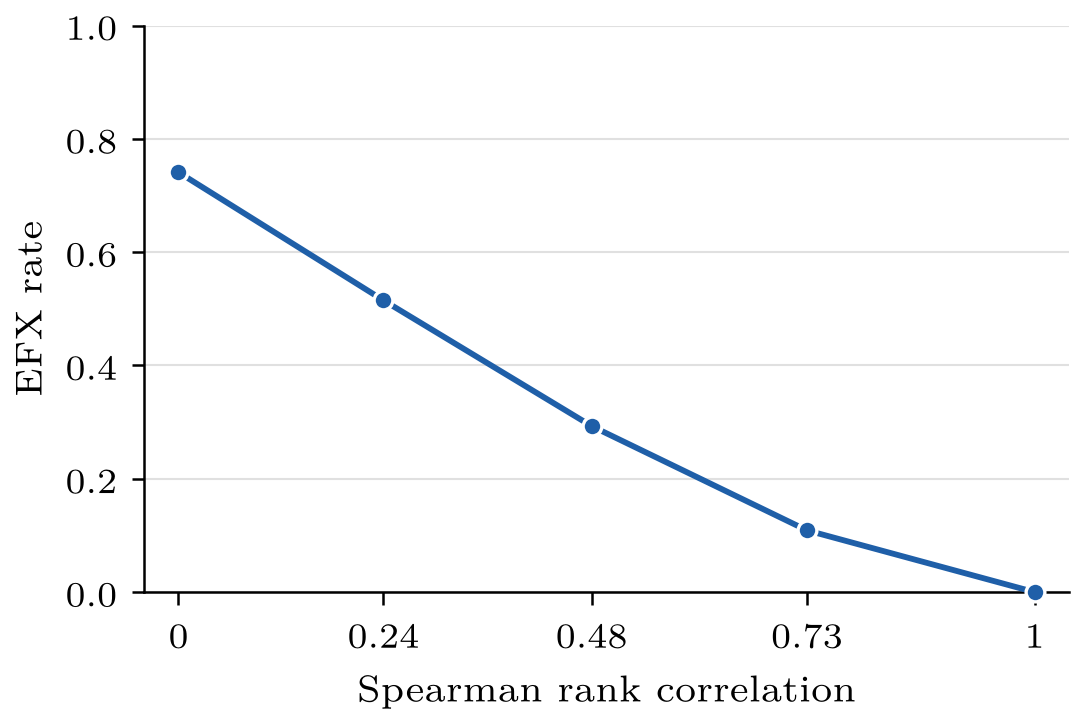
\includegraphics[width=0.6\linewidth]{agreement_rate.png}
    \caption{EFX rate of Round Robin against the Spearman rank correlation of the world from which
instances are drawn, for $n=4$ agents, $m=12$ goods and Gini $0.52$ ($\theta=1$).
Each point rests on $R=20{,}000$ instances.}
    \label{fig:placeholder}
\end{figure}

